\documentclass{article}

\usepackage{graphicx}
\usepackage[spanish]{babel}
\usepackage{minted}
\usepackage{xcolor}
\usepackage{subfig}
\usepackage{braket}
\usepackage[spanish]{babelbib}
\usepackage[utf8]{inputenc} %puse este paquete para que el Kile me ponga las ñ`s y acentos
\usepackage{amsmath}
\graphicspath{ {images/} }

\definecolor{LightGray}{gray}{0.9}
%New colors defined below
\definecolor{codegreen}{rgb}{0,0.6,0}
\definecolor{codegray}{rgb}{0.5,0.5,0.5}
\definecolor{codepurple}{rgb}{0.58,0,0.82}
\definecolor{backcolour}{rgb}{0.95,0.95,0.92}

\begin{document}

\title{Resolución del problema de la moneda falsa utilizando un algoritmo cuántico}
\author{Federico Marcos\\
\normalsize\it Departamento de Física, Universidad Nacional de La Plata}
\date{}
\maketitle

\begin{abstract}
En el presente trabajo se discute el problema de hallar una moneda de menor peso entre otras a primera vista idénticas utilizando una balanza de platos.
Se describe el algoritmo óptimo clásico y el número mínimo de pesadas necesarias para luego compararlo con un algoritmo cuántico con el mismo propósito. Se analiza la implementación del último y los resultados obtenidos utilizando un simulador de computadora cuántica. Se verifica que utilizando el algoritmo cuántico en lugar del clásico se obtiene una importante mejora en la cantidad de operaciones necesarias para hallar la moneda falsa.
\end{abstract}


% - abstract, robar de https://arxiv.org/pdf/1009.0416.pdf
% - motivacion
% - problema clasico, complejidad algoritmica, comparacion con el algo cuantico
% - descripcion del algoritmo:
%     - encoding de la query
%     - efecto de la quantum balance
%     - eleccion del estado blanco
%     - proceso de filtrado de estados con hamming weight par para usar como input
%     - comentar quantum amplitude amplification?
%     - comentar el reversing si fallo el paso anterior
%     - implementacion de una quantum balance con un CNOT
%     - transformada de hadamard para detectar la moneda falsa, sacar la demo del paper
%     - 
% - codigo del algoritmo, descripcion de cada paso
% - resultados para varios tamanios del problema
% - breve descripcion de la QC de IBM, problemas en la implementacion fuera del simulador
% - Conclusiones

\section*{Descripción del problema clásico}

El problema de la moneda falsa  fue propuesto por E.D.Schell en la edición de enero de 1945  de American Mathematical Monthly. El acertijo preguntaba si dadas 8 monedas a simple vista iguales, podemos determinar cual es la falsa ( de menor peso) únicamente utilizando una balanza de platos dos veces.
La respuesta es positiva  y despierta interés en estudiar el caso general, dadas $n$ monedas hallar el número mínimo de pesadas necesarias para determinar la falsa. También puede generalizarse para el caso de $k$ monedas falsas en un número $n$ total de monedas. Estas situaciones matemáticas fueron discutidas y resueltas clásicamente por diversos autores \cite{1}.  A continuación se discute el caso de una única moneda falsa más liviana que las otras con un total de 8 monedas.

Clásicamente podemos resolver el problema de estudio realizando dos pesadas como las que se muestra en la figura  \ref{fig:1}.
\begin{center}
    
\begin{figure}[h]
    \centering
    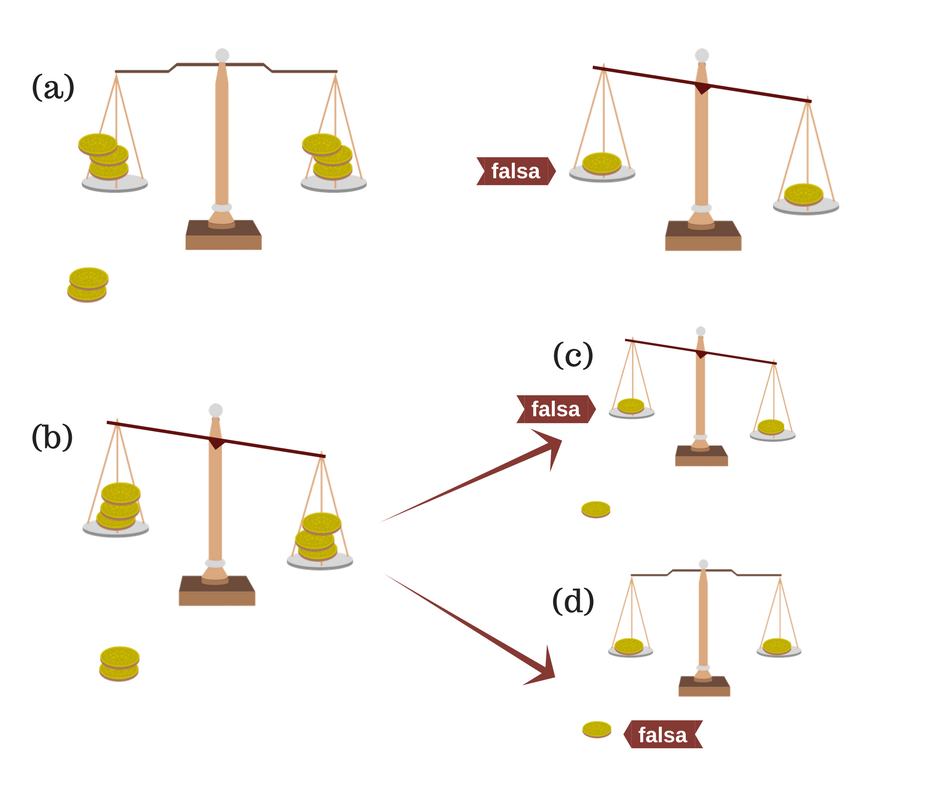
\includegraphics[scale=0.5]{img/falsa(1).png}
    \caption{Resolución del problema clásico}
    \label{fig:1}
\end{figure}
\end{center}

La primer pesada nos permite decidir si la moneda falsa esta en la balanza o no. Si la balanza no se inclina(a), la moneda falsa se encuentra entre las dos fuera de la balanza. En ese caso la segunda pesada sera entre esas dos, determinando a la más liviana como falsa.
En el caso de que en la primer pesada la balanza se incline (b), tomamos el grupo de 3 monedas más liviano, que incluye la falsa, y comparamos dos de estas dejando una afuera. Si la balanza se inclina la más liviana es la falsa (c) , si en cambio las dos son iguales (d) la falsa es la que esta fuera de la balanza. 

En k usos de la balanza podemos verificar $3^k$ monedas. Con dos pesadas podríamos identificar a la falsa entre hasta $3^2=9$ monedas, con tres pesadas podríamos encontrar la falsa entre hasta $3^3=27$ monedas etc.
En general, clásicamente,  podemos encontrar la moneda falsa en $log_3(n)$ redondeado al siguiente entero pesadas. 

Es interesante preguntarnos si la mecánica cuántica puede ofrecer una mejora en la cantidad de operaciones necesarias para encontrar la moneda falsa. 

\section*{Algoritmo cuántico}

Las computadoras cuánticas han demostrado ser capaces de resolver algunos problemas más rápidamente que cualquier computadora clásica. Podemos resaltar una reducción en la dificultad ( de exponencial a polinomial \cite{2}) en el factoreo en números primos y en la búsqueda en base de datos desestructuradas \cite{3} (de orden cuadrático) entre otros.

Se presenta a continuación el algoritmo de detección de moneda falsa en el que la información en una base de datos cuántica es analizada por una única consulta. Este es una aplicación del problema de paridad de Berstein y Vazirani \cite{4} que muestran claramente el poder de la computación cuántica .

En un algoritmo clásico cada pesada o consulta representa comparar igual número de monedas en ambos lados de la balanza, la diferencia y mejora que presenta un algoritmo cuántico es que podemos consultar una superposición de estados a la vez. Para consultar a la balanza cuántica usamos una representación binario que indica que monedas están en la balanza con un 1, la consulta 01101010 significa que las monedas con índice 1,2,4,6 están en la balanza mientras que la consulta 01110111 significa que todas las monedas menos las de índice 0 y 4 están en la balanza (el primer elemento tiene índice 0). No nos preocupa como están ubicadas las monedas en la balanza, ya que el arreglo solo nos responde equilibrada (en el caso en que la falsa no esté en la balanza) o desequilibrada ( en el caso en que la falsa esté en la balanza) .
Supongamos que la moneda falsa es la de índice 3, la consulta 01101010 va a responder equilibrada (o 0) y la consulta 01110111 va a responder desequilibrada (o 1). Se utilizan dos registros, el primero cuenta con tantos qubits como monedas y almacena la información de que monedas se incluyen en la pesada. El segundo registro se utiliza como blanco de la operación de medida cambiando el  signo del estado dependiendo el resultado de la misma. Podemos escribir una consulta a la balanza (omitiendo normalizaciones) como:

  \begin{align}
\ket{01101010}(\ket{0}-\ket{1}) \xrightarrow{Balanza \hspace{5} cuántica} \ket{01101010}(\ket{0 \oplus0}-\ket{1\oplus0})=\\
\nonumber   \ket{01101010}(\ket{0}-\ket{1}) \\
\nonumber\\
\ket{01110111}(\ket{0}-\ket{1}) \xrightarrow {Balanza \hspace{5}cuántica} \ket{01110111}(\ket{0 \oplus1}-\ket{1\oplus1})=\\
\nonumber (-1)\ket{01110111}(\ket{0}-\ket{1}) 
  \end{align}

notemos que se obtendrá un signo negativo únicamente en el caso en que la moneda falsa se encuentre sobre la balanza.

De manera general se puede escribir la acción de la balanza cuántica cuando se busca la moneda falsa entre n monedas.
  \begin{align}
\ket{x}(\ket{0}-\ket{1}) \xrightarrow {Balanza \hspace{5} cuántica} \ket{01101010}(\ket{0 \oplus0}-\ket{1\oplus0})=\\
\nonumber (-1)^{x \cdot e_k}\ket{x}(\ket{0}-\ket{1})
  \end{align}


donde x es un estado de $n$ qubits y $e_k$ el estado que tiene todos 0 salvo un 1 en el índice de la moneda falsa.

Es importante resaltar que la balanza acepta como consulta únicamente estados que tienen un número par de 1, es decir, al igual que en la balanza clásica ponemos igual número de monedas en cada plato. De otra forma no sería necesario que este presente la moneda falsa para obtener ''desequilibrado'' como respuesta.

Se prepara entonces una superposición de todos los posibles estados con un número par de unos. Para eso necesitamos un circuito que realice la operación


\begin{equation}
\ket{0} ^n\rightarrow{} \frac{1}{2^{\sqrt{(N-1)}}}\sum_{x_{par}}\ket{x} 
\end{equation} 

Dónde la suma es sobre todos los estados x de $n$ dígitos binarios con número total de unos par. La normalización proviene de que la cantidad de estados con un número par de monedas es  $2^n/2$. Se define el Hamming weight de una cadena binaria como la suma módulo dos de todos los componentes. De esta manera un estado con un número de monedas impar tendrá un Hamming weight igual a 1 y 0 en caso contrario.
Para obtener esa superposición particular se parte de un estado $\ket{0}$ y se aplican compuertas Hadamards para obtener la superposición $\sum_{x} \ket{x}$ sobre estados x con cualquier número de unos. A continuación se separan los estados con número total de unos par e impar utilizando que $(x_1+x_2+x_3...+x_n)mod_2$ dará 0 o 1 como resultado dependiendo el caso. Para realizar la suma utilizamos el operador $XOR_x$ que se implementa como una serie de operaciones $CNOT$ en cascada utilizando el primer registro como control y el segundo como blanco, acumulando en este la suma módulo 2 de los valores de cada qubit del primer registro ( ver \ref{fig:2})
Es decir, se realiza la siguiente operación:

\begin{equation}
\ket{0}\ket{0} \xrightarrow{H}\frac{1}{2^{N/2}}\sum_x\ket{x}\ket{0}\xrightarrow{XOR_x}\frac{1}{2^{N/2}}\sum_x \ket{x}\ket{0+x_1+x_2+...x_n}
\end{equation}


se puede separar los resultados obtenidos en el lado derecho de la ecuación  con respecto al resultado del $XOR$ 

\begin{equation}
\frac{1}{2^{(N-1)/2}}\sum_{|x|=0_{mod2}}\ket{x}\ket{0}+\frac{1}{2^{(N-1)/2}}\sum_{|x|=1_{mod2}}\ket{x}\ket{1}
\end{equation}

donde la suma sobre $|x|=0_{mod2}$ es sobre los estados con Hamming weight 0, y la suma sobre $|x|=1_{mod2}$ sobre los estados con Hamming weight 1.
Como ya se discutió únicamente son  válidas las consultas con un número par de unos, por ende si se mide el segundo registro y se obtiene un 0 sabremos que se están c considerando los estados apropiados y podemos proseguir a consultar la balanza cuántica. En caso contrario, se revierte el proceso aplicando Hadamards para recuperar el estado inicial y se itera hasta obtener un 0 en el segundo registro. En cada repetición tenemos una probabilidad de 1/2 de obtener el resultado deseado\footnote{es posible obtener la superposición deseada con certeza y sin necesidad de realizar una medida utilizando el mecanismo de amplificación cuántica (quantum amplitue amplification)\cite{5}}. En la figura \ref{fig:2} puede verse el circuito utilizado en caso de obtener un 1 en la medida.

\begin{figure}[h]
    \centering
    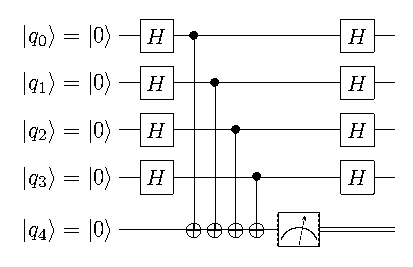
\includegraphics[scale=1.7]{img/reverse.eps}
    \caption{Circuito utilizado en caso de obtener 1 en la medida}
    \label{fig:2}
\end{figure}

Logramos entonces a través de este procedimiento construir el estado superposición de todos los posibles estados con un número par de monedas sobre la balanza, nos disponemos ahora  a construir la balanza para evaluarlos.
\subsection*{Balanza cuántica}

La balanza cuántica devuelve desequilibrada (1) si la moneda falsa está presente en la consulta,es decir si el estado contiene un 1 en el índice de la moneda falsa y 0 en caso contrario, siendo únicamente capaz de evaluar estados con un número par de unos.
Si llamamos k al índice de la moneda falsa, la balanza  no hace más que dada la consulta $\ket{x_1,x_2,...x_n}\ket{0}$ devolver $\ket{x_1,x_2,...x_n}\ket{0\oplus x_k}$ que puede realizarse con un CNOT entre el segundo registro y el $x_k$ .
Es decir la acción de la balanza  sobre el estado superposición es:

\begin{align}
    \ket{x_1,x_2,...x_n}(\ket{0}-\ket{1}) \xrightarrow{Balanza \hspace{5} cuántica}\ket{x_1,x_2,...x_n}(\ket{0\oplus x_k}-\ket{1\oplus x_k})=\\
    \nonumber (-1)^{x\cdot e_k}\ket{x_1,x_2,...x_n}(\ket{0}-\ket{1})
\end{align}

Esta última consideración nos permite construir un operador cuántico capaz de evaluar una superposición de consultas simultáneamente y a su vez emular la capacidad de identificar a la moneda falsa por sobre el resto.


\subsection*{Identificación de la moneda falsa}

Una vez obtenida la respuesta de la balanza se procede a identificar la moneda falsa aplicando la transformada de Hadamard en el primer registro obteniendo el siguiente esquema

\begin{align}
    &\frac{1}{2^{(N-1)/2}}\sum_{|x|=0_{mod2}}\ket{x} \xrightarrow{Balanza \hspace{5} cuántica} \frac{1}{2^{(N-1)/2}}\sum_{|x|=0_{mod2}}(-1)^{x\cdot e_k}\ket{x} \\
    & \frac{1}{2^{(N-1)/2}}\sum_{|x|=0_{mod2}}(-1)^{x\cdot e_k}\ket{x}\xrightarrow{H^N} \frac{1}{\sqrt 2}(\ket{e_k}+\ket{\hat{e_k}})
\end{align}
donde $e_k$ es un estado con todos 0 salvo un 1 en el lugar k y $\hat{e_k}$ es un estado con todos 1 salvo un 0 en el lugar k. El ultimo paso se debe a que si aplicamos la transformada de Hadamard se obtiene

\begin{align*}
    H\ket{x}&=\frac{1}{2^{(n-1)/2}}\sum_{|x|=0_{mod2}}(-1)^{x\cdot e_k}H\ket{x}\\
    &=\frac{1}{2^{n-1}\sqrt{2}}\sum_{|x|=0_{mod2}}\sum_{z\in \{0,1\}^n}(-1)^{x\cdot (e_k+z)}\ket{z}\\
    &= \frac{1}{\sqrt{2}}\left(\ket{e_k} + \ket{\hat{e_k}}\right) + \frac{1}{2^{N-1}\sqrt{2}}\sum_{|x|=0 _{mod2}}\hspace{5}\sum_{z \neq e_k, \hat{e_k}}(-1)^{x\cdot(e_k+z)}\ket{z}\\
    &= \frac{1}{\sqrt{2}}\left(\ket{e_k} + \ket{\hat{e_k}}\right)
\end{align*}

Notar que la ultima igualdad se satisface dado que el segundo término debe anularse  considerando que el primero ya tiene norma uno.

Al medir y colapsar el estado en una de estas dos posibilidades se es capaz de identificar el índice de la moneda falsa ya que en cualquiera de los dos casos será distinto a los demás.

En la figura \ref{fig:3} puede verse el circuito completo

\begin{center}
\begin{figure}[h]
    \centering
    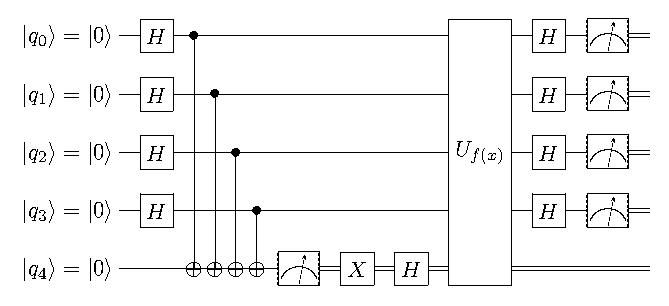
\includegraphics[scale=1]{img/circ.eps}
    \caption{Circuito completo utilizado en caso de obtener 0 en la medida intermedia. $U_f(x)$ representa a la balanza cuántica.}
    \label{fig:3}
\end{figure}
\end{center}

\section*{ Descripcion de IBM QISKit}
El algoritmo anteriormente mencionado puede ser corrido en diferentes entornos como los proporcionado por IBM Quantum Information Software Kit (QISKit) \cite{6}.
Este permite crear diferentes programas cuánticos, compilarlos y ejecutarlos en uno de los distintos entornos disponibles como simuladores locales, simuladores en la nube y procesadores cuánticos de 5 y 16 qubits con distinta arquitectura. La red de IBM Q cuenta con implementaciones de computadora cuántica basadas en el comportamiento de superconductores. Para cualquier implementación de qubit, los estados cuánticos lógicos $\{\ket{0},\ket{1}    \}$ se mapearán a los diferentes estados físicos del sistema, típicamente a niveles de energía discretos (cuantificados) o a sus superposiciones cuánticas. Para el qubit de carga, los diferentes niveles de energía corresponden a un número entero de pares de Cooper en una isla superconductora. Para el qubit de flujo, los niveles de energía corresponden a números enteros diferentes de cuantos de flujo magnético atrapados en un anillo superconductor. Para el qubit de fase, los niveles de energía corresponden a diferentes amplitudes de oscilación de carga cuántica a través de la unión Josephson, donde la carga y la fase son análogas al momento y la posición correspondientemente de un oscilador armónico cuántico.


Para el caso de 1 moneda falsa entre 8 se necesita un número mínimo de 9 qubits. El procesador ibmqx5 (de 16 qubits) de IBM presenta las siguientes características:
La conectividad de la red esta proporcionada por un total de 22 cavidades resonantes coplanares (CPW), cada uno de los cuales conecta 2 qubits. La configuración de conexión se puede observar en la figura \ref{fig:4}. Los puntos coloreados representan qubits, y las barras indican resonadores CPW. Se utilizan tres diferentes frequencias de resonancia, las barras blancas indican cavidades con 6.25 GHz, las grises de 6.45GHz y las negras de 6.65GHz.

\subsection*{Compuertas binarias}
Todas las compuertas de dos qubits y sus direcciones estan definidas en un mapa de acoplamiento y se pueden observar en la figura \ref{fig:6}. En general, compuertas de dos qubits son posibles entre qubits vecinos que esten conectados por un superconductor resonante. IBM Q experience usa la interacción cross-resonancia como la base para la compuerta Control NOT. Esta interacción es más intensa cuando se elije el qubit con mayor frecuencia como control, y el qubit de menor frecuencia como blanco, por lo que las frecuencias de los qubits determinan las direcciones de las compuertas.
Dadas las anteriores limitaciones es a menudo necesario compilar el programa el cual automatiza la aplicación de una secuencia de compuertas SWAP que propagan la operación de control a qubits no vecinos, y a su vez transforman las operaciones necesarias en otras equivalentes de manera que sean compatibles con la configuración geométrica. A pesar de esto, al momento de escribir este informe los procesadores cuánticos reales no cuentan con un mecanismo de feedback que permita utilizar la sentencia condicional $c\_if$, por lo que se procede a hacer un estudio utilizando el simulador local.

\begin{center}
\begin{figure}[H]
    \centering
    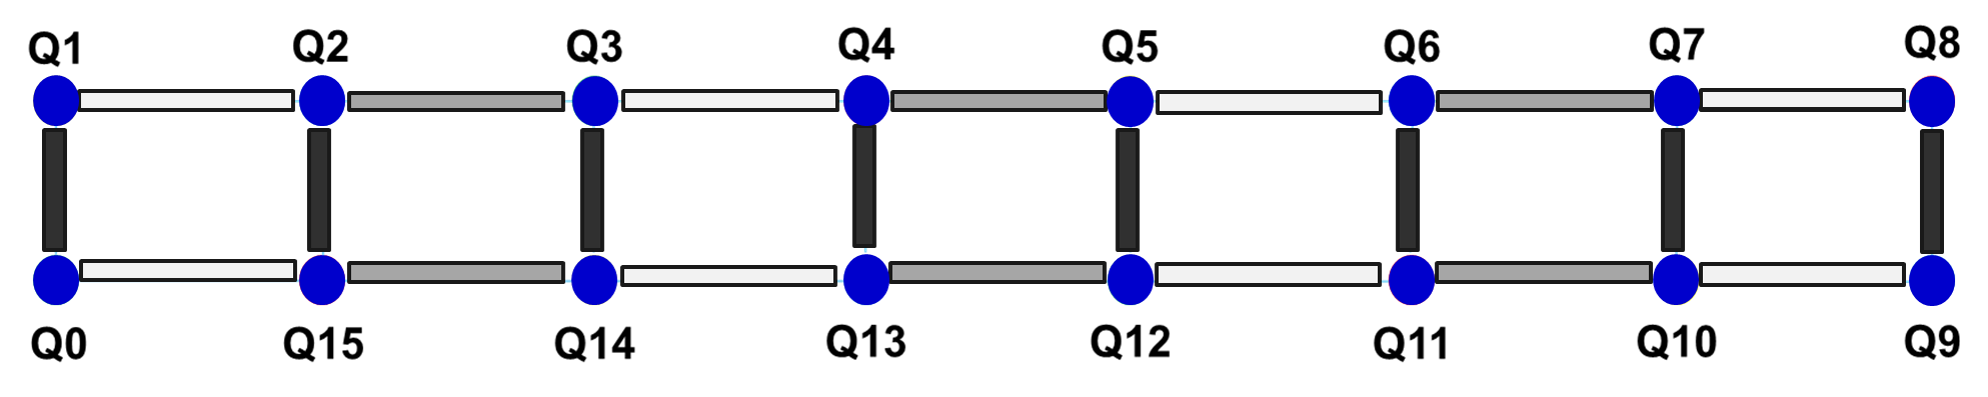
\includegraphics[scale=0.25]{img/ibmqx3-bus.png}
    \caption{Diagrama de conexión de ibqx3}
    \label{fig:4}
\end{figure}
\end{center}


\begin{center}
\begin{figure}[H]
    \centering
    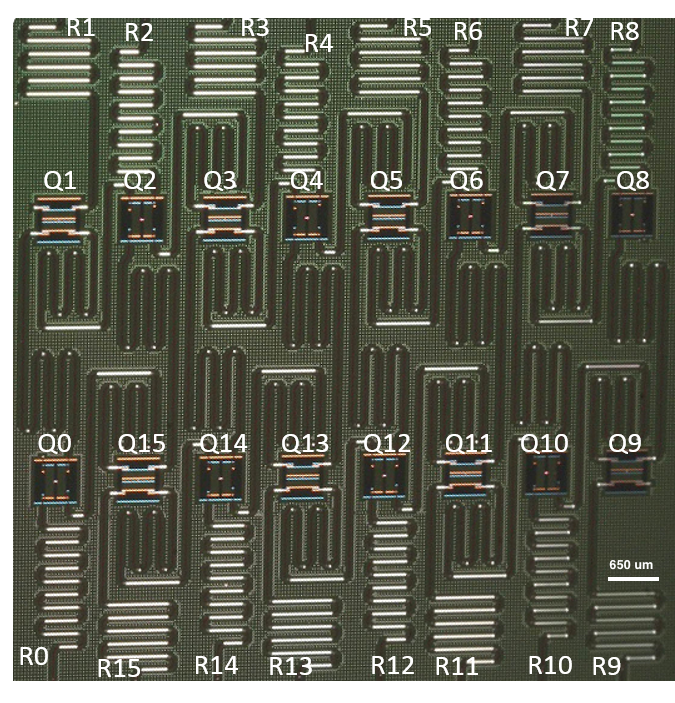
\includegraphics[scale=0.4]{img/ibmqx3-labeled.png}
    \caption{Disposición de los qubits en el chip}
    \label{fig:5}
\end{figure}
\end{center}

\begin{center}
\begin{figure}[H]
    \centering
    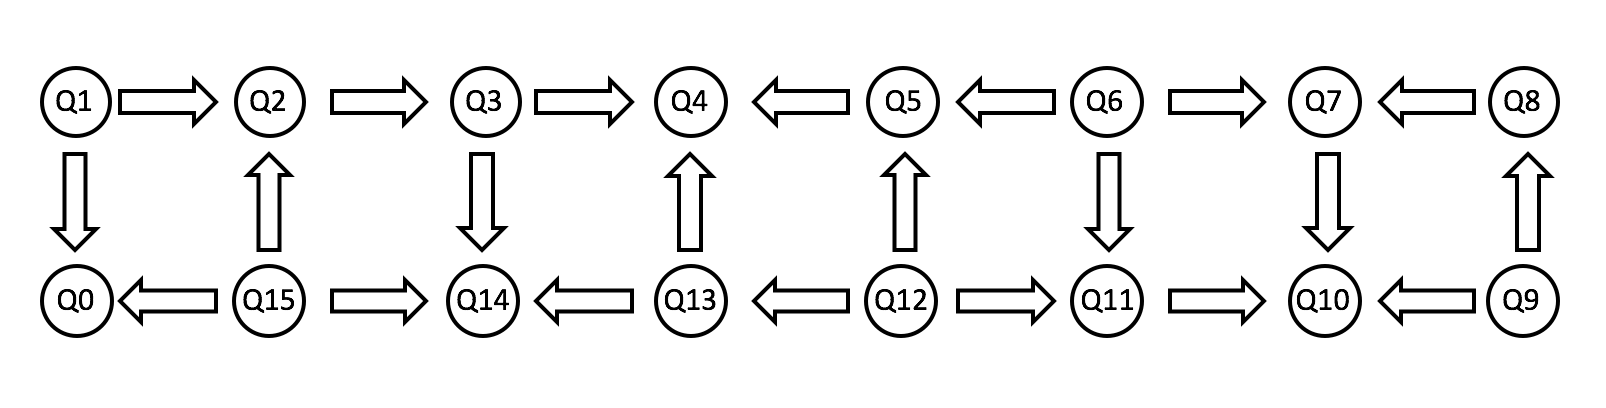
\includegraphics[scale=0.5]{img/IBMQX5_connections_full.png}
    \caption{Mapa de acoplamiento}
    \label{fig:6}
\end{figure}
\end{center}

\section*{Código del algoritmo}

A continuación se describe el código utilizado para detectar la moneda falsa en un simulador de computadora cuántica
Se importan las librerías necesarias para interactuar con QISkit y graficar los resultados:
\begin{minted}
[
framesep=2mm,
baselinestretch=1.2,
bgcolor=LightGray
]{python}
import sys
import matplotlib.pyplot as plt
%matplotlib inline
import numpy as np
from math import pi, cos, acos, sqrt
from qiskit import QuantumProgram
import Qconfig
from qiskit.tools.visualization import plot_histogram
\end{minted}
\\
Se definen las variables del problema:
\\
\begin{minted}[
framesep=2mm,
baselinestretch=1.2,
bgcolor=LightGray
]{python}
# Máximo número de qubits disponibles
M = 16             
# Este número debería ser menor o igual a M-1, 
# donde M es el numero de qubits disponibles
numberOfCoins = 8   
# Esto deberia ser 0, 1, ..., numberOfCoins - 1
indexOfFalseCoin = 6     

if numberOfCoins < 4 or numberOfCoins >= M:
    raise Exception("""Please use numberOfCoins
        between 4 and """, M-1)
if indexOfFalseCoin < 0 or indexOfFalseCoin >= numberOfCoins:
    raise Exception("""indexOfFalseCoin must be between 
        0 and """, numberOfCoins-1)
\end{minted}
\newpage

Se crea un programa y se define la configuración del circuito:

\begin{minted}[
framesep=2mm,
baselinestretch=1.2,
bgcolor=LightGray
]{python}
Q_program = QuantumProgram()
# seteo dek APIToken y API url
Q_program.set_api(Qconfig.APItoken, Qconfig.config["url"]) 

# Creando los registros
# numberOfCoins qubits para el string binario de búsqueda
# y 1 qubit for para trabajar y almacenar el resultado 
# de la balanza cuántica
qr = Q_program.create_quantum_register("qr", numberOfCoins+1)
# para almacenar las medidas sobre qr
cr = Q_program.create_classical_register("cr", numberOfCoins+1)

circuitName = "QueryStateCircuit"
queryStateCircuit = Q_program.create_circuit(circuitName,
    [qr], [cr])

N = numberOfCoins
# Creamos una superposición uniforme de todos las 
# cadenas de caracteres de largo N
for i in range(N):
    queryStateCircuit.h(qr[i])

# Realizamos un XOR(x) aplicando compuertas CNOT secuencialmente 
# desde qr[0] hasta qr[N-1] y guardando el resultado en qr[N]
for i in range(N):
    queryStateCircuit.cx(qr[i], qr[N])

# Medimos qr[N] y guardamos el resultado en cr[N]. 
# El algoritmo continúa si cr[N] es cero,
# o se repite de otra manera
queryStateCircuit.measure(qr[N], cr[N])

# Se procede a consultar a la balanza cuántica 
# si el valor de cr[0]...cr[N] son todos cero
# preparando el estado de Hadamard |1>, i.e., |0> - |1> en qr[N]
queryStateCircuit.x(qr[N]).c_if(cr, 0)
queryStateCircuit.h(qr[N]).c_if(cr, 0)

# deshacemos el cómputo cuando cr[N] no es cero
for i in range(N):
    queryStateCircuit.h(qr[i]).c_if(cr, 2**N)

\end{minted}




Como ya discutimos se emula la balanza cuántica usando una compuerta CNOT con el índice de la moneda falsa:

\begin{minted}[
framesep=2mm,
baselinestretch=1.2,
bgcolor=LightGray
]{python}
k = indexOfFalseCoin
# Aplicamos la balanza cuántica al estado superposición deseado
queryStateCircuit.cx(qr[k], qr[N]).c_if(cr, 0)
\end{minted}


Para identificar la moneda falsa, se aplica la transformada de Hadamard

\begin{minted}[
framesep=2mm,
baselinestretch=1.2,
bgcolor=LightGray
]{python}
# Aplicamos la transformada de Hadamard a qr[0] ... qr[N-1]
for i in range(N):
    queryStateCircuit.h(qr[i]).c_if(cr, 0)

# Medimos qr[0] ... qr[N-1]
for i in range(N):
    queryStateCircuit.measure(qr[i], cr[i])
\end{minted}


Podemos realizar un histograma con los resultados:

\begin{minted}[
framesep=2mm,
baselinestretch=1.2,
bgcolor=LightGray
]{python}
# Este backend es un simulador de procesador cuántico
backend = "local_qasm_simulator"
# Número de veces a repetir el experimento
shots = 200 
results = Q_program.execute([circuitName], 
    backend=backend, shots=shots)
answer = results.get_counts(circuitName)
valid_answer = {key:val for key,val in answer.items() 
    if key[0:1] == "0"}
plot_histogram(valid_answer)

from collections import Counter
for key in valid_answer.keys():
    normalFlag, _ = Counter(key[1:]).most_common(1)[0] 
    for i in range(2,len(key)):
        if key[i] != normalFlag:
            print("False coin index is: ", len(key) - i - 1)
\end{minted}
\section*{Resultados}

Utilizando el programa anterior se tiene una probabilidad de 50\% de obtener la superposición de estados con Hamming weight par y proceder al algoritmo de pesado. En este caso, al completar el proceso el bit de la izquierda será 0 y el resto contendrá números idénticos excepto en el índice de la moneda falsa \footnote{notar que se numera de derecha a izquierda comenzando con 0}. En el caso en que la moneda de índice 6 sea la falsa se obtiene con igual probabilidad uno de los siguientes resultados para los registros clásicos donde se almacenan los resultados de las mediciones: $010111111$ o $001000000$. Esto puede observarse en la figura \ref{fig:7}

\begin{center}
\begin{figure}[H]
    \centering
    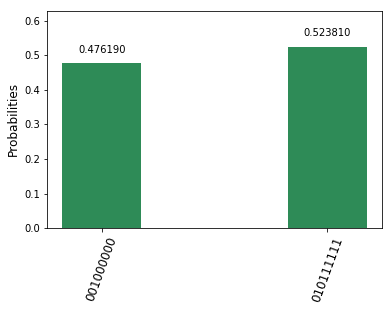
\includegraphics[scale=0.7]{img/histograma.png}
    \caption{Resultado para 8 monedas}
    \label{fig:7}
\end{figure}
\end{center}
Comparando los 8 dígitos correspondientes concluimos que el índice de la moneda falsa es el 6 en ambos casos, como esperábamos.

Es posible variar el número de monedas del algoritmo, pero el tiempo de cómputo y la cantidad de memoria necesaria para la simulación crece exponencialmente con el número de qubits\footnote{ Los tiempos de procesamiento del simulador fueron de menos de un segundo por consulta en el caso de 8 qubits y de menos de un minuto por consulta en el caso de 20 qubits, creciendo el tiempo de manera exponencial con el número de qubits}. En la figura \ref{fig:8} se ve un ejemplo con 20 monedas.
\begin{center}
\begin{figure}[H]
    \centering
    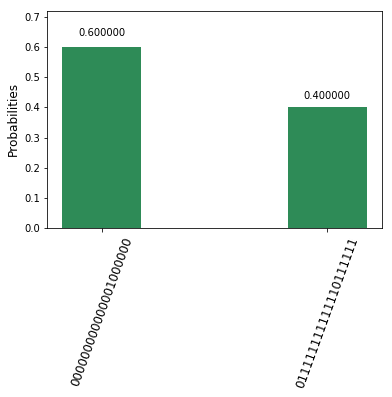
\includegraphics[scale=0.7]{img/historgama2.png}
    \caption{20 monedas}
    \label{fig:8}
\end{figure}
\end{center}

\section*{Conclusiones}

 Se discutió en profundidad el problema de la moneda  falsa en un total de 8 monedas con un algoritmo cuántico. Utilizando un simulador de computadora cuántica se verificó (para el caso de una moneda falsa) la reducción en la cantidad de consultas a la balanza, de orden logarítmico respecto al número de monedas en el caso clásico a una única consulta en el caso cuántico. Se muestra el código necesario para implementar el algoritmo.
 El problema analizado es de gran importancia ya que este algoritmo junto con otros, muestran el  indiscutible potencial de la computación cuántica.

\begin{thebibliography}{}
\bibitem{1}J. Dominguez-Montes ; Solution to the Counterfeit Coin Problem and its Generalization
 \texttt{https://arxiv.org/pdf/1005.1391.pdf}
\bibitem{2}J.P.W. Shor, “Algorithms for quantum computation: discrete
log and factoring,” Proceedings of the 35th Annual
Symposium on the Foundations of Computer Science
(IEEE Computer Society Press, Los Alamitos, CA
1994), p. 124.
\bibitem{3}L.K. Grover, “A fast quantum mechanical algorithm for
database search,” Proceedings of the 28th Annual ACM
Symposium on Theory of Computing, 1996, pp. 212-219.
\bibitem{4}E.Bernstein, U.Vazirani, “Quantum complexity theory”,
Proceedings of the 25th Annual ACM Symposium on
Theory of Computing, 1993, pp.11-20.
\bibitem{5}Gilles Brassard, Peter Hoyer, Michele Mosca, Alain Tapp "Quantum Amplitude Amplification and Estimation"
    \texttt{https://arxiv.org/abs/quant-ph/0005055v1}
\bibitem{6}Quantum Information Software Kit
\texttt{https://www.qiskit.org/}
\bibitem{7}azuo Iwama, Harumichi Nishimura, Rudy Raymond, Junichi Teruyama "Quantum Counterfeit Coin Problems"
\texttt{https://arxiv.org/pdf/1009.0416.pdf}
\bibitem{8}Barbara M. Terhal and John A. Smolin "Single quantum querying of a database"
\texttt{https://arxiv.org/pdf/quant-ph/9705041.pdf}
\end{thebibliography}
\end{document}
